\documentclass[a4paper,12pt]{article}

\RequirePackage{epsfig}

\setlength\hoffset{-0.5in}      %% these work quite well with a 12pt font
\setlength\voffset{-0.5in}
\setlength{\textwidth}{6.30in}
\setlength{\textheight}{9.0in}

\bibliographystyle{unsrt}

\usepackage{xcolor}
\newcommand{\ajs}[1]{\textcolor{orange}{[AJS: #1]}}
\newcommand{\note}[1]{\textcolor{red}{#1}}
\newcommand{\mk}
[1]{\textcolor{blue}{[MK: #1]}}


\begin{document}

\begin{center}
{\Large\bf{Towards Evaluating Creativity in Language}} \\
      \vspace{5.0mm}
{\Large\bf{Project Plan}} \\
      \vspace{8mm}
      {\large\bf{Matey Krastev}}  \\
      \vspace{5.0mm}
       {\tt m.krastev.19@abdn.ac.uk} \\
      \vspace{5.0mm}
      {\em Department of Computing Science,\\
       University of Aberdeen, Aberdeen AB24 3UE, UK} 
\end{center}


\section*{Introduction}

Large language models (LLMs) are probabilistic models of language that widely used for most tasks in the field of Natural Language Processing (NLP), ranging from machine translation, text classification, sentiment analysis, auto-completion, error correction, or even simple dialogue communication. However, because, fundamentally, LLMs operate on probabilities, a lot of the applications utilizing them tend to struggle with generating logically coherent novel sequences. 

Large language models are usually trained on enormous language corpora, mined from books and articles\cite{gutenberg_dataset}, social media posts\cite{broad_twitter}, or otherwise internet crawls.\cite{thepile_dataset}. Therefore the underlying assumption would be that, in their attempt to replicate language, they could find some success at least in terms of generating basic structure in creative fields of work such as writing code\cite{codex_2021_copilot} or screenplays\cite{mirowski_co-writing_2022}, among others. 
% vv tbh after the however part it sounds weird vv
% \ajs{Maybe the flow of the following paragraph can be started with: While LLMs display convincingly human-like text in many areas, this thesis aims to evaluate the extent to which, we can evaluate their output in terms of its \textit{creativity}. This research question is by nature subjective, thus a starting point is to examine which characteristics of human-written creative texts differ from more structured, and thus less creatively oriented genres e.g. news articles, or writing where the aim is to concisely communicate factual information. Having identified specific linguistic markers within human-written creative texts, we can then begin to evaluate the extent to which LLMs exhibit these properties in generated text. This in turn has the potential to inform techniques to adapt existing model generation for applications involving creative language such as writing tools. As a first step towards this goal, this thesis will explore and develop automatic measures to predict and evaluate the creativity of a text...  }

However, this would then beg the question of whether the creativity they exhibit can be classified as conventional human creativity, and if so, which specific linguistic markers define human creativity. We, therefore, argue that a more unified benchmark needs to be defined for creativity evaluation and classification. 

% The impact of large language models (LLMs) in recent years cannot be understated. 
% Language models are finding their way in nearly every task imaginable, thanks to incremental improvements in the quality of prompt answers, suggestions and code tips. Some people even tend to use prompt-based models to answer their specific questions, in a way akin to how search engines operated in recent years. 

% A model assisting workers in high-level abstraction jobs, such as those in creative writing, code development, medical practice and what are generally fields which require deep expertise in a variety of topics and enormous knowledge bases, can potentially spark a productivity boom similar to the ones experienced during the invention of semiconductors.

% Most current language models, therefore, are trained on massive datasets comprising data almost on the order of magnitude of all resources available on the world wide web. Some would argue [[maybe insert ref]] that this would prove more than enough to satisfy the needs of the everyday consumer. However, defining one such LLM as artificial intelligence would largely neglect one of the most essential factors of human intelligence - creativity. 

% Evaluating and benchmarking creativity is a task that has already been undertaken by researchers [[insert ref]] with varying degrees of success owing to the very abstract definition of the term itself. This project, therefore, seeks to compile and produce a software package that can efficiently, and more importantly, accurately represent creativity in language, or more formally, linguistic creativity. 

\section*{Goals}
We set out to investigate specific markers defining or correlating with conventional creativity in language. As some aspects of creativity have been investigated by research disciplines such as the field of psycholinguistics 
% this is nice, however it's not necessary in the plan, we can use it for the thesis instead.
% \ajs{e.g. patterns of part of speech use, use of concrete vs. abstract concepts \cite{brysbaert2014concreteness}, patterns of information density\cite{giulianelli2021analysing}, use of complex vs simple vocabulary \cite{kuperman2012age} etc.}, 
we seek to filter and compile a set of measures that have been shown to correlate more highly with creative texts in the literature. 
Following that, we aim to evaluate the extent to which current LLMs can provide insights into capturing creative elements or patterns within writing. Finally, if time allows, we may use these findings to explore how natural language generation can be adapted to produce texts exhibiting more human-like levels of the creative attributes we have discovered. These can be summarised by the following three questions:

\begin{itemize}
    \item Can psycho-linguistically motivated measures (that is, the explored metrics) successfully characterise creative properties in language?
    \item Can a machine learning approach be adapted for evaluating creativity in natural language?
    \item Can we influence a subset of current LLMs to exhibit more creative traits as defined by our creativity metric via some conventional approaches such as hyperparameter tuning or varying decoding strategies? 
\end{itemize}

For the first two, we develop a suite of benchmarks we shall distribute and report the results of. 
For the third question, we plan to train a model maximising performance on the developed benchmarks. We will then report our findings on the best-performing models and share the architecture.

% In other words, describe \emph{what} it is that you want to do.
% Are you building a tool or an application? What functionality 
% already exists, and what will you have to do yourself?

% Try to make it clear which goals are central to your project, and which
% might be optional extras. Try to be realistic about making your
% goals {\em achievable.}


\section*{Methodology}
A major part of the project will be spent on research and iterative development of the metrics and benchmarks. This is a process that requires analysing and compiling resources on creative aspects of writing and language overall. As part of addressing question two, we plan to train and evaluate a classifier based on these features. 
Another major factor will be the development time spent on measuring the creativity of existing language models. We choose to utilise the Transformer-based machine learning architecture\cite{vaswani_attention_2017} for some of the metrics we shall develop. 

\subsection*{Dataset Collection}
The initial progress will be dataset collection and storage. In order to perform larger-scale testing, we require clean and structured data. Therefore, we will: prepare and clean the data; apply normalisation techniques such as unknown word discounting and filtering filler words; apply parts of speech (POS) tagging via tools such as the NLTK package for Python\cite{nltk_citation}. 

Datasets to be used include: the ROC and Cloze Test dataset\cite{mostafazadeh-etal-2016-corpus}; the Project Gutenberg corpus of 50,000 books\cite{gutenberg_dataset}, and the Lexical Database for English ``Wordnet"\cite{wordnet_princeton}. More potential resources may be used if the scope of the project allows.

\subsection*{Metric Compilation and Creation}
Some groundwork has already been put forth in the field of creativity research (e.g. patterns of part of speech use, use of concrete vs. abstract concepts \cite{brysbaert2014concreteness}, patterns of information density\cite{giulianelli2021analysing}, use of complex vs simple vocabulary \cite{kuperman2012age}), however, no effort has been done to systematically compile and create benchmarks. 
We set out to collect, filter and produce a set of benchmarks. We choose to implement those in the Python programming language as a command-line utility. Of course, we reserve some time to test and debug the benchmarks to ensure production-level quality.


\subsection*{Machine Learning Approaches}
Later stages of the project will require the use of machine learning frameworks. The currently preferred approach is using high-level abstractions in the Python programming language with bindings for highly-optimized parallelisable data structures implemented in commonly fast programming languages such as C/C++. Thus, we opt to apply PyTorch library\cite{NEURIPS2019_9015_pytorch}, which implements such GPU-accelerated machine learning development, wherever high-performance computing is desired. 

We plan to make use of existing pre-trained LLMs such as GPT\cite{brown_gpt3_2020} and OPT\cite{zhang_opt_2022} to evaluate the extent to which they can generate human-like creative text, then (optional) in subsequent experiments explore the extent to which varying parameters during generation can induce more human-like patterns.

% % vv is this needed or can you cut it? vv
% Neural network-based models tend to contain a very high number of trainable parameters, usually having a net size on the order of hundreds of millions of weights. These models need to be moved to a high-performance computing cluster, as even a high-end personal computer would not be able to handle having those in memory, let alone perform the number crunching in a reasonable time frame. 
% %
% \newline Therefore, We have outlined a high-level overview of the tasks as follows: 
% %A relatively high-level view of the development process would be:


% %% give examples/cite some authors for these to show that you have already done some research
% \begin{itemize}
% \item compiling and consulting available literature on the matter of creativity;
% \item developing a systematic and rigorous set of benchmarks for aspects of conventional creativity exhibited in human-produced text and speech;
% \item testing and fine-tuning the developed benchmarks;
% \item exploring approaches to influence exhibited creativity in LLMs; as part of this, we may perform larger-scale testing on HPC clusters;
% \end{itemize}
% %

\section*{Resources Required}
A mid- to high-end personal computer would be required for prototyping the metric, as well as building the interface and tools to interact with the system.
To develop the creativity measures, we require a sizable and clean dataset as outlined above.  
Furthermore, a high-performance computing (HPC) cluster will be needed for utilising the large language models which have been open-sourced for research and general purposes. 
Python will be our programming language of choice.

An ethics review will not be required, as the project does not deal with human subjects. 

\section*{Risk Assessment}

The only major risks that threaten the successful execution of the project are schedule-based. The project is fundamentally research-intensive. Currently, we have mitigated this risk by carefully considering a schedule and goals outlined week by week. The schedule takes into account the author's capabilities.
%and seeks to not place a heavy burden on them during the project execution. 
Frequent meetings with the project supervisor serve to check on the progress achieved in the past week, as well as to clarify the deliverables for the upcoming one. Through strict adherence to the timetable outlined below, we minimise the risks against the successful execution of the project. 

Additionally, we acknowledge the scope-related risks. Depending on the project load and the progress from week to week, we run the risk of lagging behind schedule for the final task of creative text generation: as training a model tends to take a long time even on an HPC cluster, we need to be mindful of the limits the HPC cluster itself puts forward on usage. As an external factor, we may mitigate the risk by backing up the progress made in training the model, for example. Another risk related to the usage of the HPC cluster, albeit minor, could be an experienced heavy load as other students and staff may attempt to run computations during the same time, which could slow down the training time more. Still, this final task is detached from the key goals of the project, so even in the worst case, failure to accomplish it does not endanger the overall completion of the project.   
 % *ramble* yth do i need to explain all risks, if i describe a risk, it should probably be something critical not minor annoyances
% \ajs{I agree with your comment in the text here, this section does seem less necessary, but good job, it looks well written to me. if you struggle for space, this part can be compressed in my opinion.}

\begin{figure}[htb!]
\begin{center}
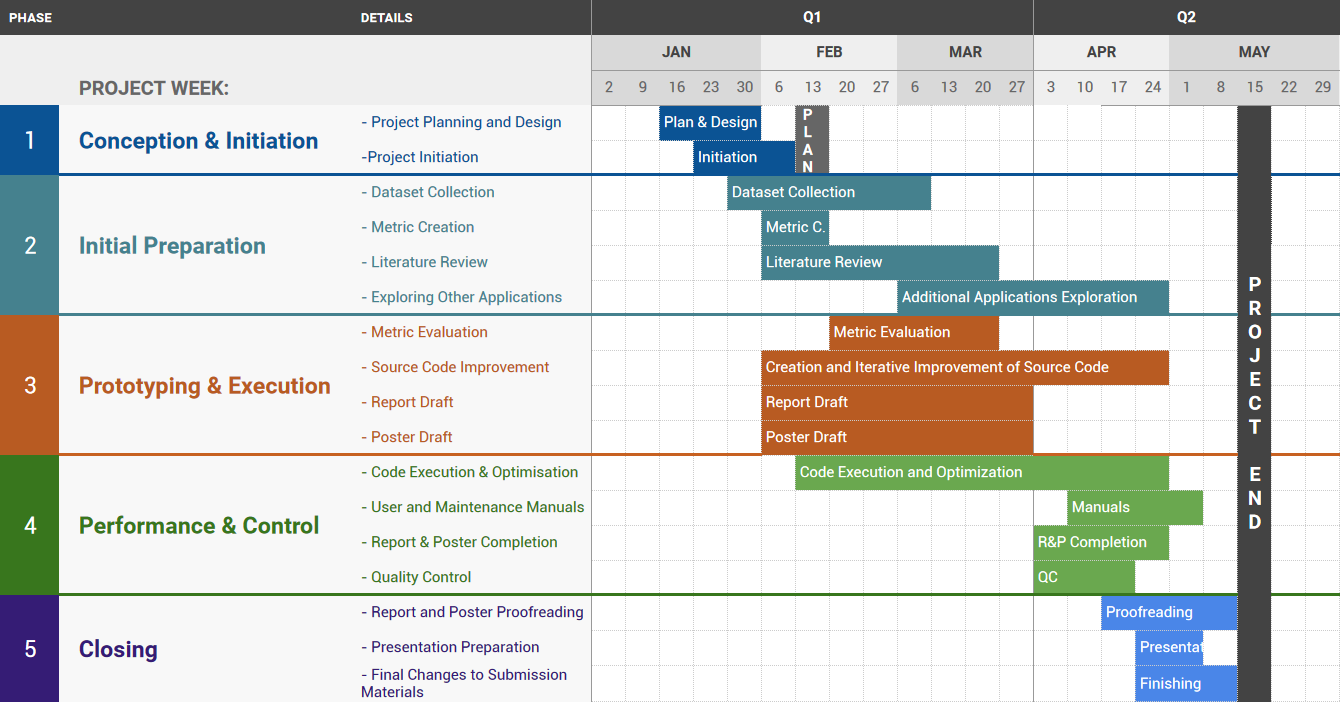
\includegraphics[width=\textwidth]{plan.png}
\caption{Timetable for Main Project Activities \label{fig:plan}}
\end{center}
\end{figure}

\section*{Timetable}
Outlined in Figure~\ref{fig:plan} is a brief overview of the expected deliverables for each week until the final deadline for the project.

% For information, this figure was created using xfig, and 
% converted to encapsulated postscript by a command in the Makefile
% before being included as a graphic in the \LaTeX document.

\bibliography{ProjectPlan}

\end{document}
